%% start of file `cv_german.tex', based on `template_en.tex` by Xavier Danaux (xdanaux@gmail.com).
% This work may be distributed and/or modified under the
% conditions of the LaTeX Project Public License version 1.3c,
% available at http://www.latex-project.org/lppl/.
% 
% Thomas Quaritsch <t.quaritsch@student.tugraz.at>

\documentclass[11pt,a4paper]{moderncv}
\usepackage[german]{babel}
\usepackage{moderncv-additions}
\usepackage{pdfpages}
\usepackage{url}

% moderncv themes
\moderncvtheme{casual}   % optional arguments are 'blue' (default), 'orange', 'red', 'green', 'grey' and 'roman' (for roman fonts, instead of sans serif fonts)
%\moderncvtheme[green]{classic}                % idem

% character encoding
\usepackage[utf8]{inputenc}                   % replace by the encoding you are using

% adjust the page margins
\usepackage[scale=0.8]{geometry}
\setlength{\hintscolumnwidth}{3cm}			  % if you want to change the width of the column with the dates
%\AtBeginDocument{\setlength{\maketitlenamewidth}{6cm}}  % only for the classic theme, if you want to change the width of your name placeholder (to leave more space for your address details


\AtBeginDocument{\recomputelengths}           % required when changes are made to page layout lengths

% personal data
\firstname{Simon}
\familyname{Szustkowski}
%\title{Resumé title (optional)}               % optional, remove the line if not wanted
\address{Marsbruchstraße 117}{44287 Dortmund}        % optional, remove the line if not wanted
\mobile{+49 176 24692840}                     % optional, remove the line if not wanted
\phone{+49 231 3306614}                      % optional, remove the line if not wanted
%\fax{fax (optional)}                          % optional, remove the line if not wanted
\email{mail@simonszu.de}                      % optional, remove the line if not wanted
%\extrainfo{additional information (optional)} % optional, remove the line if not wanted
\photo[64pt]{picture}                          % '64pt' is the height the picture must be resized to and 'picture' is the name of the picture file; optional, remove the line if not wanted
%\quote{``Das ist ein toller Frusterspruch\\ von Friede Frusterfrau.'' -- Friede Frusterfrau}                 % optional, remove the line if not wanted

%\nopagenumbers{}                             % uncomment to suppress automatic page numbering for CVs longer than one page


%----------------------------------------------------------------------------------
%            content
%----------------------------------------------------------------------------------

\begin{document}

% color redefinitions must be after \begin{document}!
\definecolor{firstnamecolor}{RGB}{125,85,85}
\definecolor{familynamecolor}{RGB}{138,74,57}
\definecolor{quotecolor}{RGB}{125,85,85}
\definecolor{addresscolor}{RGB}{125,85,85}
\definecolor{sectionrectanglecolor}{RGB}{138,74,57}
\definecolor{sectiontitlecolor}{RGB}{138,74,57}
\definecolor{subsectioncolor}{RGB}{125,85,85}
\definecolor{footersymbolcolor}{RGB}{125,85,85}	

\makeatletter

\pagestyle{empty}
\chapter*{Curriculum }{Vitae}

\vspace*{50mm}
\begin{minipage}{\textwidth}
	\vspace*{3mm}
	\familynamestyle{\@firstname}~~\firstnamestyle{\@familyname} 	
	\hspace*{5mm}{{\color{firstnamecolor}\includegraphics[width=64pt]{picture}}}\\[3mm]
	\@addressstreet, \@addresscity ~~~ \mobilesymbol~\@mobile ~~~ \emailsymbol~\@email
\end{minipage}
\begin{minipage}{70pt}
	
\end{minipage}

\vfill

\begin{minipage}{1.0\textwidth}
	\section{Table of contents}
	\tableofcontents
\end{minipage}

\newpage
\pagestyle{fancy}
%\chapter{Curriculum}{~Vit\ae}
\chapter{Curriculum Vitae}{}
\makequote

\section{Personal Data}
%%%%%%%%%%%%%%%%%%%%%%%%%%%%%%%%%%%%%%%%%%%%%%%%%%%%%%%%%%%%%%%%%%%%
\cvline{Name}{\@firstname~\@familyname}
\cvline{Address}{\@addressstreet, \@addresscity}
\cvline{Phone}{\@mobile}
\cvline{E-Mail}{\@email}
\cvline{Birthday}{11.02.1988 in Münster}
\cvline{Citizenship}{Germany / Switzerland}
%\cvline{Familienstand}{ledig}
%\cvline{Präsenzdienst}{abgeleistet}
\cvline{Driver's License}{B}
\makeatother 

%\cventry{year--year}{Degree}{Institution}{City}{\textit{Grade}}{Description}  % arguments 3 to 6 are optional

\section{Education} 
%%%%%%%%%%%%%%%%%%%%%%%%%%%%%%%%%%%%%%%%%%%%%%%%%%%%%%%%%%%%%%%%%%%%

\cventry{10/2009 -- 04/2018}{Bachelor of Science}{Technical University}{Dortmund}{\textit{Computer Sciences}}{Subsidiary subject: mechanical engineering}  % arguments 3 to 6 are optional

\cventry{09/2006 -- 06/2009}{Mechatronical engineering (CIC)}{Miele \& Cie. KG}{Bielefeld}{}{Additionally: electrically qualified person} 

\section{Professional experience} 
%%%%%%%%%%%%%%%%%%%%%%%%%%%%%%%%%%%%%%%%%%%%%%%%%%%%%%%%%%%%%%%%%%%%

\cventry{01/2022 -- today}{Senior Consultant}{VIADA GmbH \& Co. KG}{Dortmund}{}{Cloud-Infrastructure and DevOps Engineering with main focus on Red Hat OpenShift and Ansible, additionally: Team Lead of the dedicated project team}
\cventry{05/2018 -- 01/2022}{Consultant}{VIADA GmbH \& Co. KG}{Dortmund}{}{Cloud-Infrastructure and DevOps Engineering with main focus on Red Hat OpenShift and Ansible}
\cventry{12/2012 -- 04/2018}{Administrator of the Wide Area Network}{ECOFIS GmbH}{Dortmund}{}{}
\cventry{10/2010 -- 11/2012}{First Level Support}{Institute for social research of the Technical University}{Dortmund}{}{}
\cventry{09/2006 -- 06/2009}{Trainee for mechatronical engineering (CIC)}{Miele \& Cie. KG}{Bielefeld}{}{}

\section{Project overview}
\cventry{04/2023 -- today}{Build-up and operations of container-based edge infrastructure}{Medium-sized company for software in industrial manufacturing}{Limburg a.d. Lahn}{}{Deliver and implement a concept for automatic provisioning and operation of OpenShift clusters which should serve software for smart manufacturing operation management at the location of the end customers}
\cventry{12/2022 -- 03/2023}{Infrastructure for a security gateway}{Globally active IT- and communication provider}{Wolfsburg}{}{Setup and handover of a cloud-based infrastructure for the operation of a security gateway for an eID-application as requested by the German Bundesdruckerei as the responsible engineer}
\cventry{04/2022 --11/2022}{Infrastructure for logistics project}{Globally active IT- and communication provider}{Wolfsburg}{}{Setup und and handover of a  cloud-based infrastructure for an application for handling digital delivery notices as the responsible architect and engineer. The system was set up in accordance to the requirements by GS1 Germany. The project could gain the first customers during a first PoC while it was still in the setup phase.}
\cventry{01/2022 -- 03/2022}{Automation VoIP}{Globally active IT- and communication provider}{Wolfsburg}{}{The setup of a jitsi-based VoIP stack was automated with the help of ansible for an end customer from the healthcare industry. We achieved a reducing of the Time-to-market from 10 to 1 working days.}
\cventry{10/2021 -- 12/2021}{Application monitoring}{Car manufacturer}{Sindelfingen}{}{Conceptualizing and implementing of a monitoring solution based on the Prometheus stack during a migration phase from bare metal to Microsoft Azure. \\ This enabled the customer, who only relied on reactive monitoring before, to identify potential incidents with the help of proactive monitoring.}
\cventry{08/2021 -- 09/2021}{Consulting Shopware as a Service}{Globally active IT- and communication provider}{Wolfsburg}{}{Lead infrastructure architect for implementing a shopware platform as a SaaS-solution on the Open Telekom Cloud \\ Technical migration of an existing shopware platform to a could-native infrastructure with consolidation of the operation team in accordance to the GDPR at the same time.}
\cventry{01/2020 -- 07/2021}{OpenShift architecture optimization}{Car manufacturer}{Munich}{}{Accompanying the end customer from the car manufacturing industry particularly with a regard on efficient agile transformation of the platform operations team with the focus point GitOps.  \\ With an engineering team we conceptualized, implemented and continually improved the agile processes so that the daily business could transform from pure problem engineering to feature engineering. To fulfull the need of better traceability and versioning of the feature deployments we introduced the usage of ArgoCD into the processes of the international operations team.}
\cventry{01/2019 -- 12/2019}{Introduction of OpenShift}{Mutual financial association}{Frankfurt a.M}{}{Technical introduction of Red Hat OpenShift with a special focus on customer specific needs regarding security and compliance in accordance with BaFin standard. \\ As a platform operation team processes were implemented to fulfill the requirements of the BaFin, especially hardening of the environments, setup of georedundant backups, collecting and analyzing the log files with a retention time of 10 years, as well as automated container and image security checks.}
\cventry{07/2018 -- 12/2018}{Installation and configuration of AppAgile on the Open Telekom Cloud}{Logistics company}{Hamburg}{}{Customer enablement for the development of container based applications, introduction of a backup process with the help of restic and the Open Telekom Cloud}

\section{Certifications}
\cventry{06/2024}{Specialist for agile leadership (IHK)}{thekey.career}{}{Zertifikats-ID: ac-2024-be5250}{}
\cventry{06/2021}{Specialist in Containers and Kubernetes}{Red Hat}{}{Certificate-ID: 200-059-038}{}
\cventry{03/2020}{Specialist in Ansible Automation}{Red Hat}{}{Certificate-ID: 200-059-038}{}
\cventry{07/2013}{IPv6 Sage}{Hurricane Electric}{}{}{}
\cventry{07/2009}{Electrically qualified person}{Chamber of Industry and Commerce}{Bielefeld}{}{}
\cventry{01/2007}{Amateur radio operator (CEPT Novice)}{German Federal Network Agency}{Münster}{}{}

\section{Languages} 
%%%%%%%%%%%%%%%%%%%%%%%%%%%%%%%%%%%%%%%%%%%%%%%%%%%%%%%%%%%%%%%%%%%%

\cvline{Deutsch}{native language}{}
\cvline{English}{fluent}
\cvline{French}{basic knowledge}
\cvline{Danish}{basic knowledge}
\cvline{Dutch}{basic knowledge}


\section{Awards} 
%%%%%%%%%%%%%%%%%%%%%%%%%%%%%%%%%%%%%%%%%%%%%%%%%%%%%%%%%%%%%%%%%%%%
\cvline{01/2022}{Viada Innovation Award 2022}
\cvline{01/2019}{Viada Subject Matter Expert in IT Automation and Management}
\cvline{01/2019}{Viada Subject Matter Expert in Hybrid Cloud Infrastructure Administration}

%\cvline{xx/xxxx}{Musterpreis}


\section{Leisure time activities} 
%%%%%%%%%%%%%%%%%%%%%%%%%%%%%%%%%%%%%%%%%%%%%%%%%%%%%%%%%%%%%%%%%%%%

\cvline{Chaostreff Dortmund e.V.}{Visiting and supporting events in the general environment of the Chaos Computer Club} 
\cvline{German Federal Agency for Technical Relief Unna-Schwerte}{Technical reliever}
\cvline{Event service Matthias van der Wal}{Technical operations of the main stages of several conventions for Anime, Manga and Nerd culture as a volunteer}

\section{Interests}
%%%%%%%%%%%%%%%%%%%%%%%%%%%%%%%%%%%%%%%%%%%%%%%%%%%%%%%%%%%%%%%%%%%%

\cvline{Ham radio operations}{Operation of an amateur radio station (CEPT Novice)}
\cvline{Photography}{Photography of landscapes and architecture}
\cvline{Making}{3D-printing and microcontroller-programming in the environment of the maker and open source scene}

\section{Profile}
\cvline{GitHub}{\url{https://github.com/simonszu}}
\cvline{Thingiverse}{\url{https://www.thingiverse.com/ttk_/designs}}
\cvline{Docker Hub}{\url{https://hub.docker.com/u/simonszu}}
\cvline{LinkedIn}{\url{https://www.linkedin.com/in/simonszu/}}
\cvline{Xing}{\url{https://www.xing.com/profile/Simon_Szustkowski}}

%\section{Publikationen} 
%%%%%%%%%%%%%%%%%%%%%%%%%%%%%%%%%%%%%%%%%%%%%%%%%%%%%%%%%%%%%%%%%%%%

%\subsection{Konferenzen und Workshops}

%\cvline{mm/jjjj}{Autor 1 und Autor 2. \textbf{Mustertitel: Unser tolles Paper.} In \textit{Proceedings of the First Muster Workshop 1970}, Musterstadt, Musterland, YYYY.}

% \newpage

%\subsection{Technical Reports}

%\cvline{....}{....}

%\cvline{....}{alternativ kann man auch BibTex verwenden:}

%\renewcommand*{\refname}{Abschlussarbeiten}
%\nocite{*}
%\bibliographystyle{cv}
%\bibliography{publications}       % 'publications' is the name of a BibTeX file


%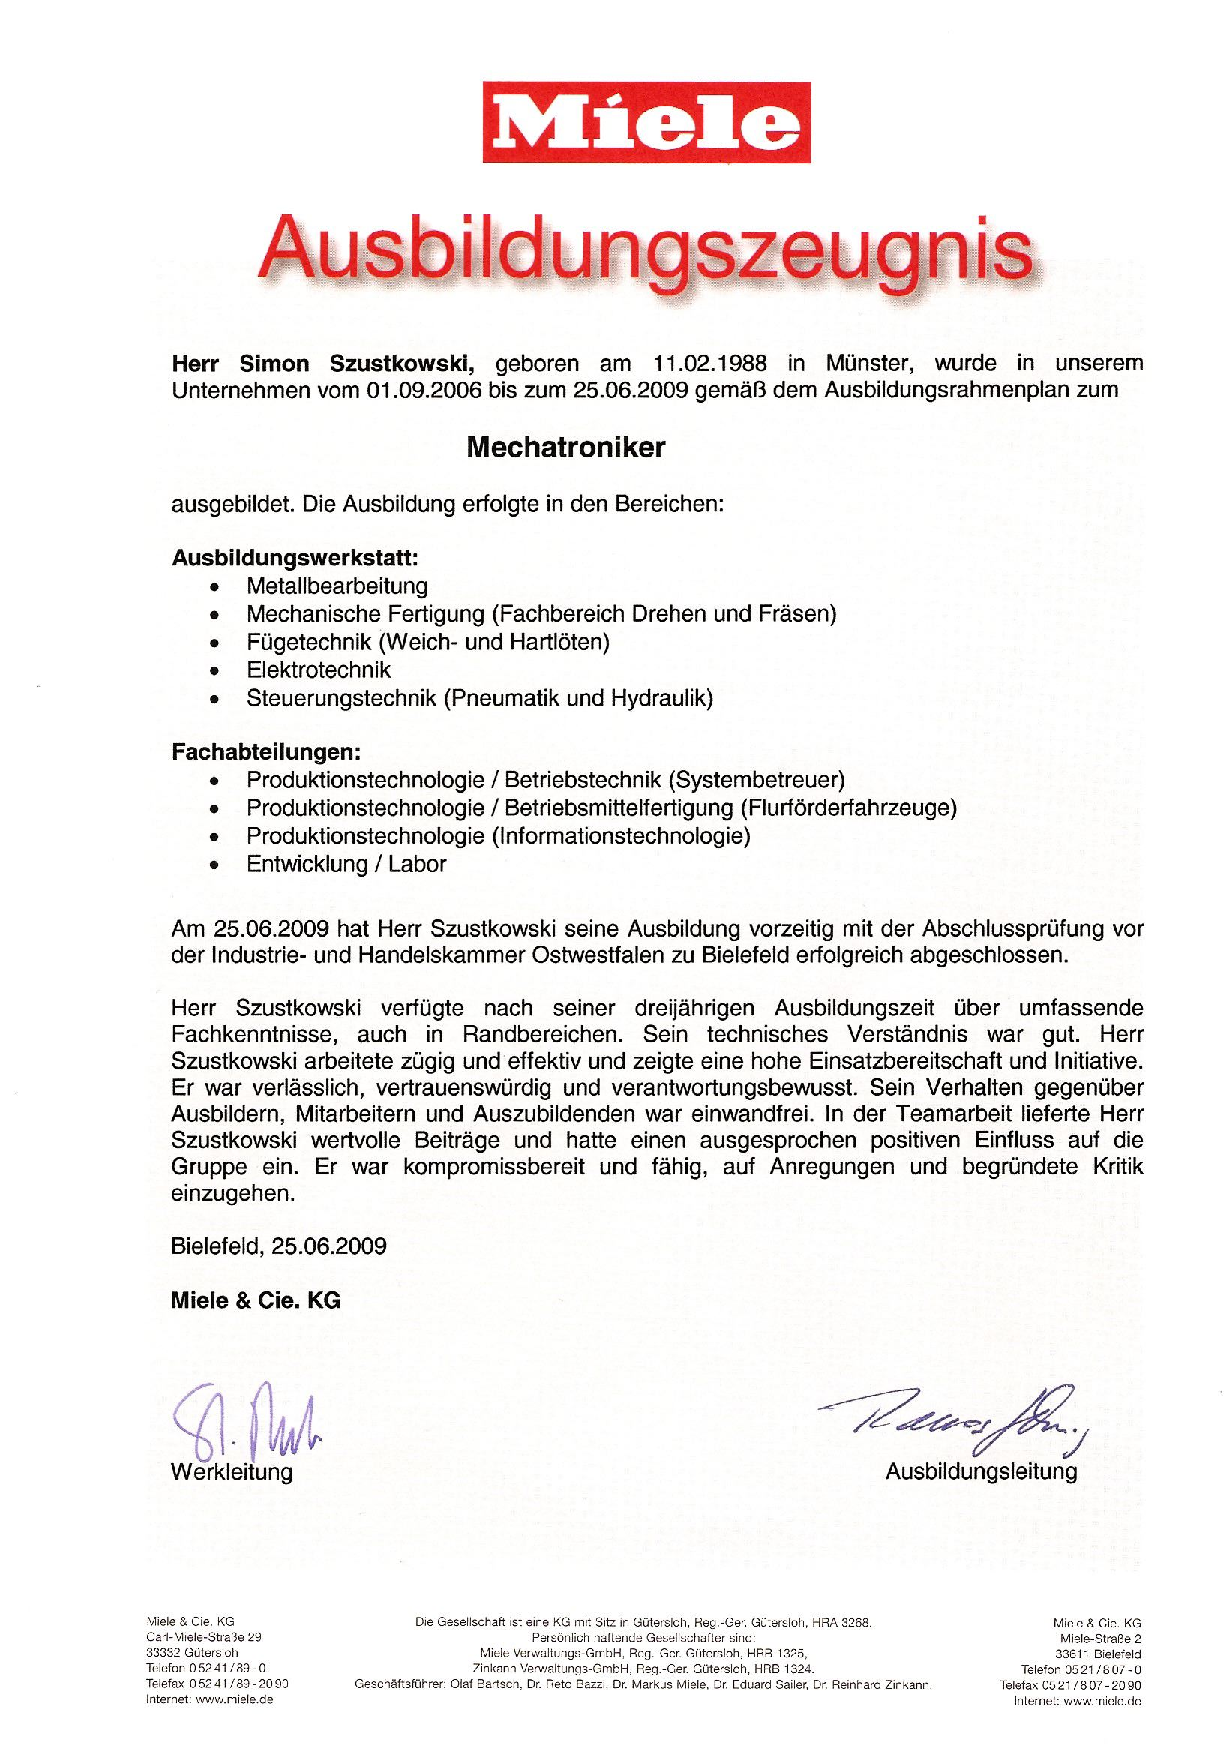
\includepdf[pages=1,addtotoc={
%	4, chapter, 1, Arbeitszeugnis Miele \& Cie. KG, az-miele
%	}]{azmiele.pdf}
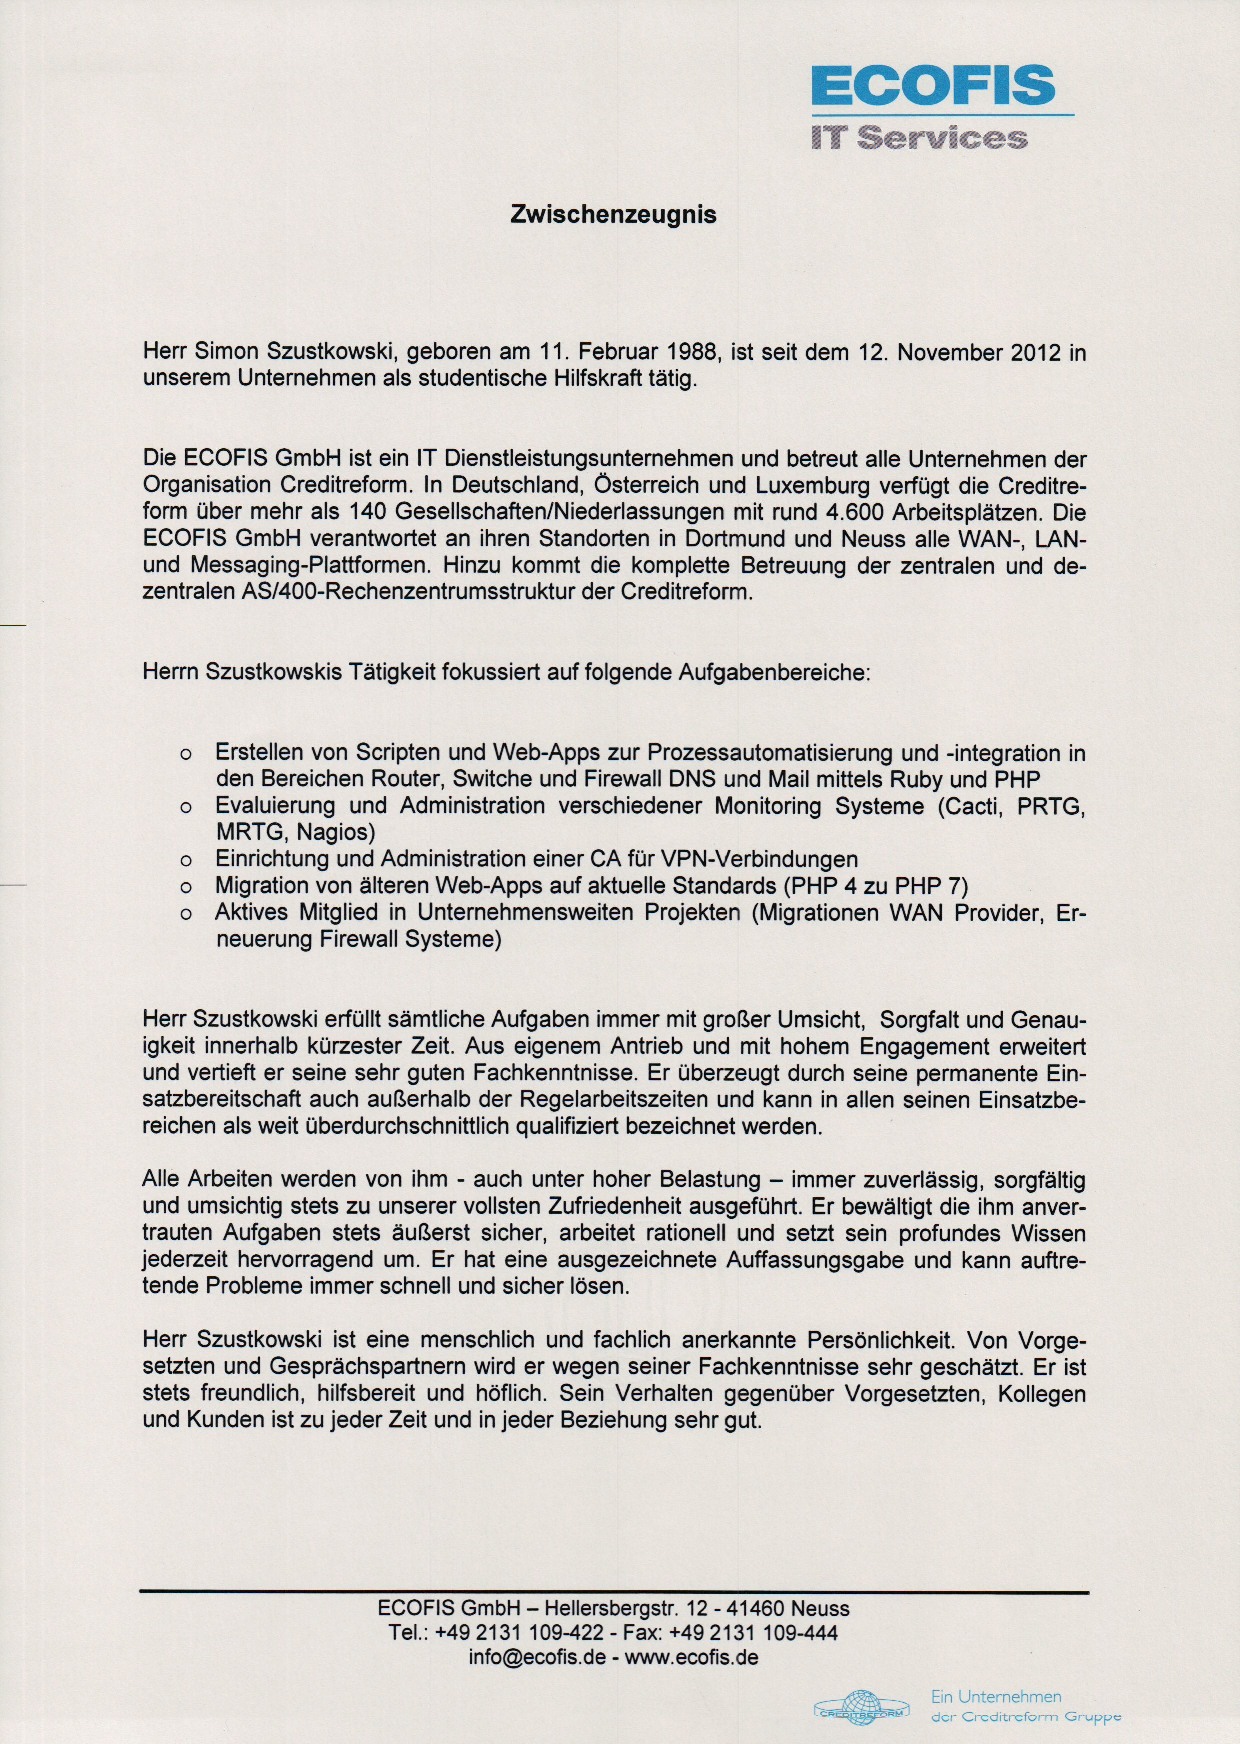
\includepdf[pages=1-,addtotoc={1, section, 1, Reference ECOFIS GmbH, azecofis} ]{./Arbeitszeugnisse/ECOFIS.pdf}
%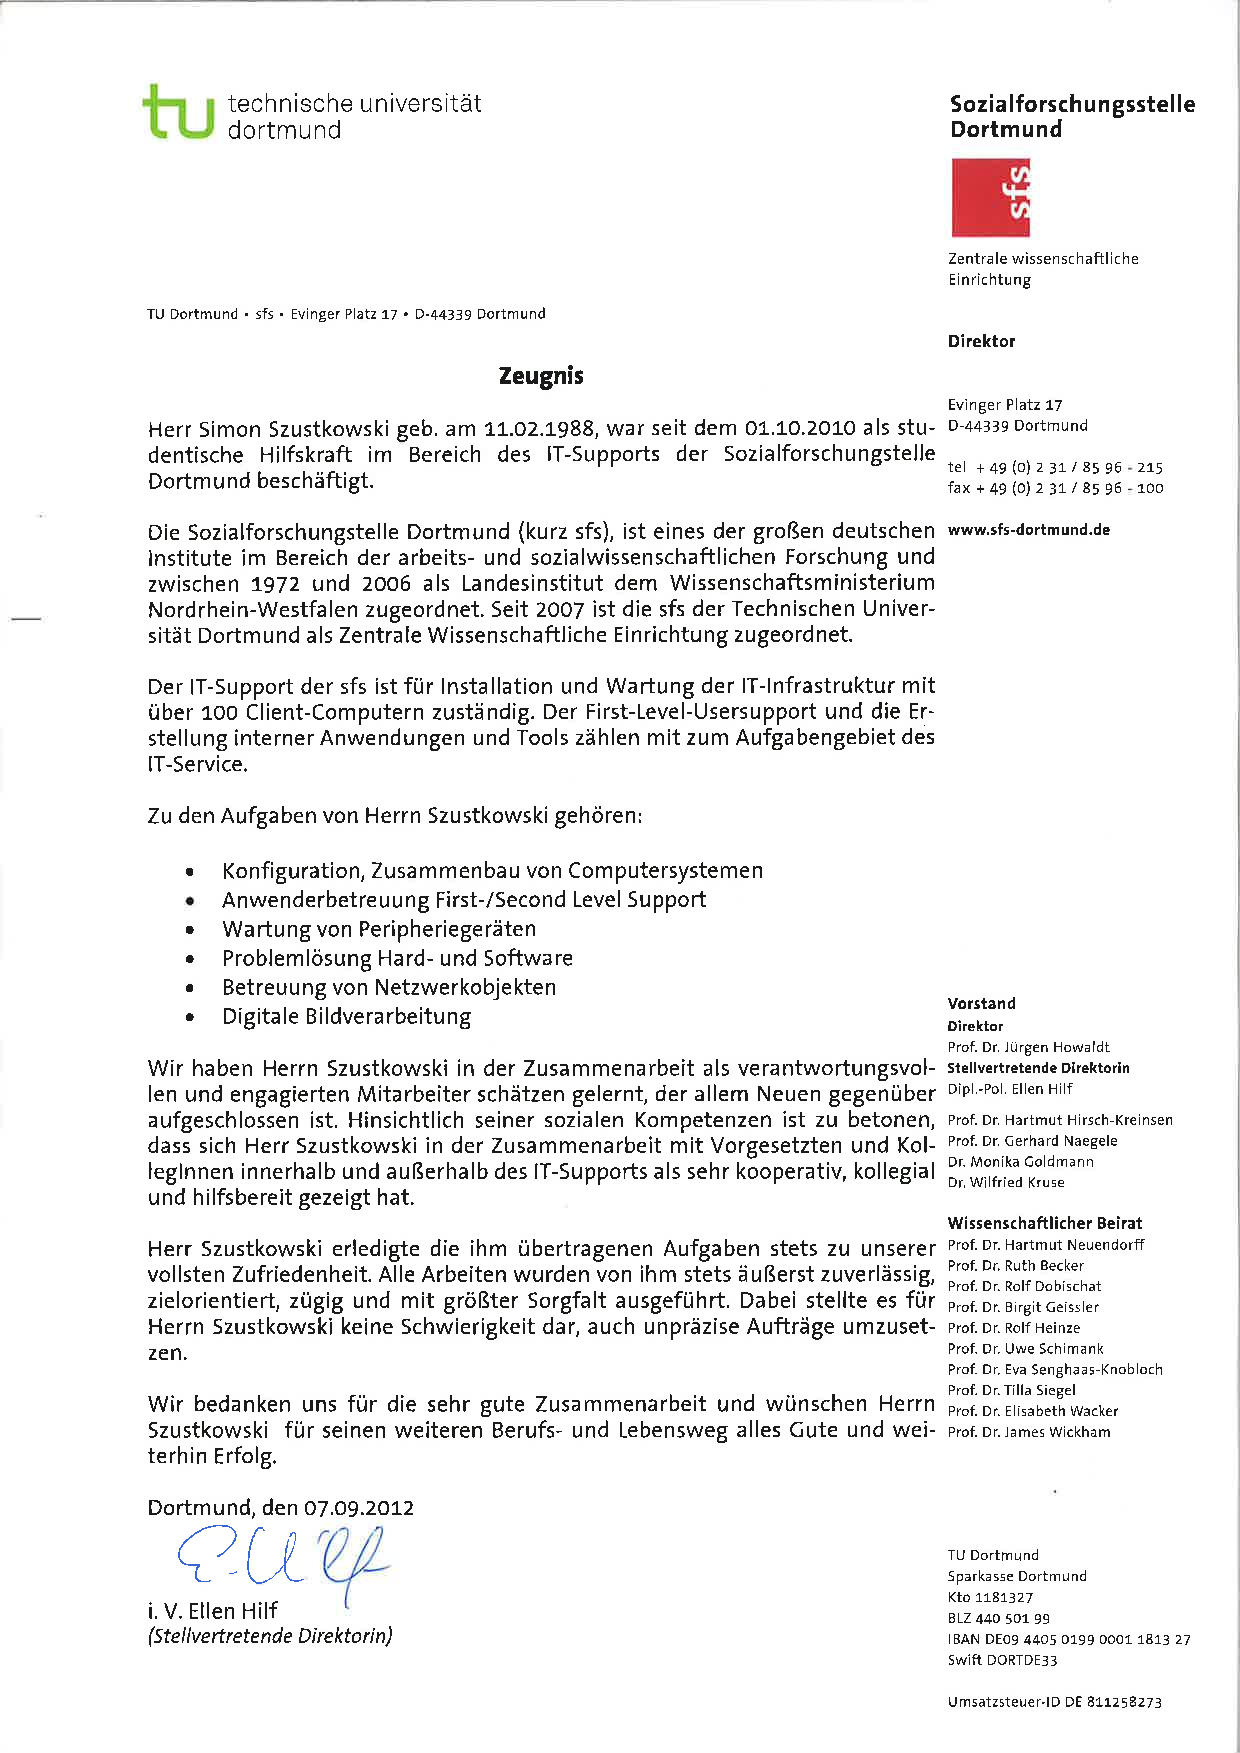
\includepdf[pages=1,addtotoc={1, section, 1, Arbeitszeugnis Sozialforschungsstelle Dortmund, azsfs} ]{./Arbeitszeugnisse/SFS.pdf}
%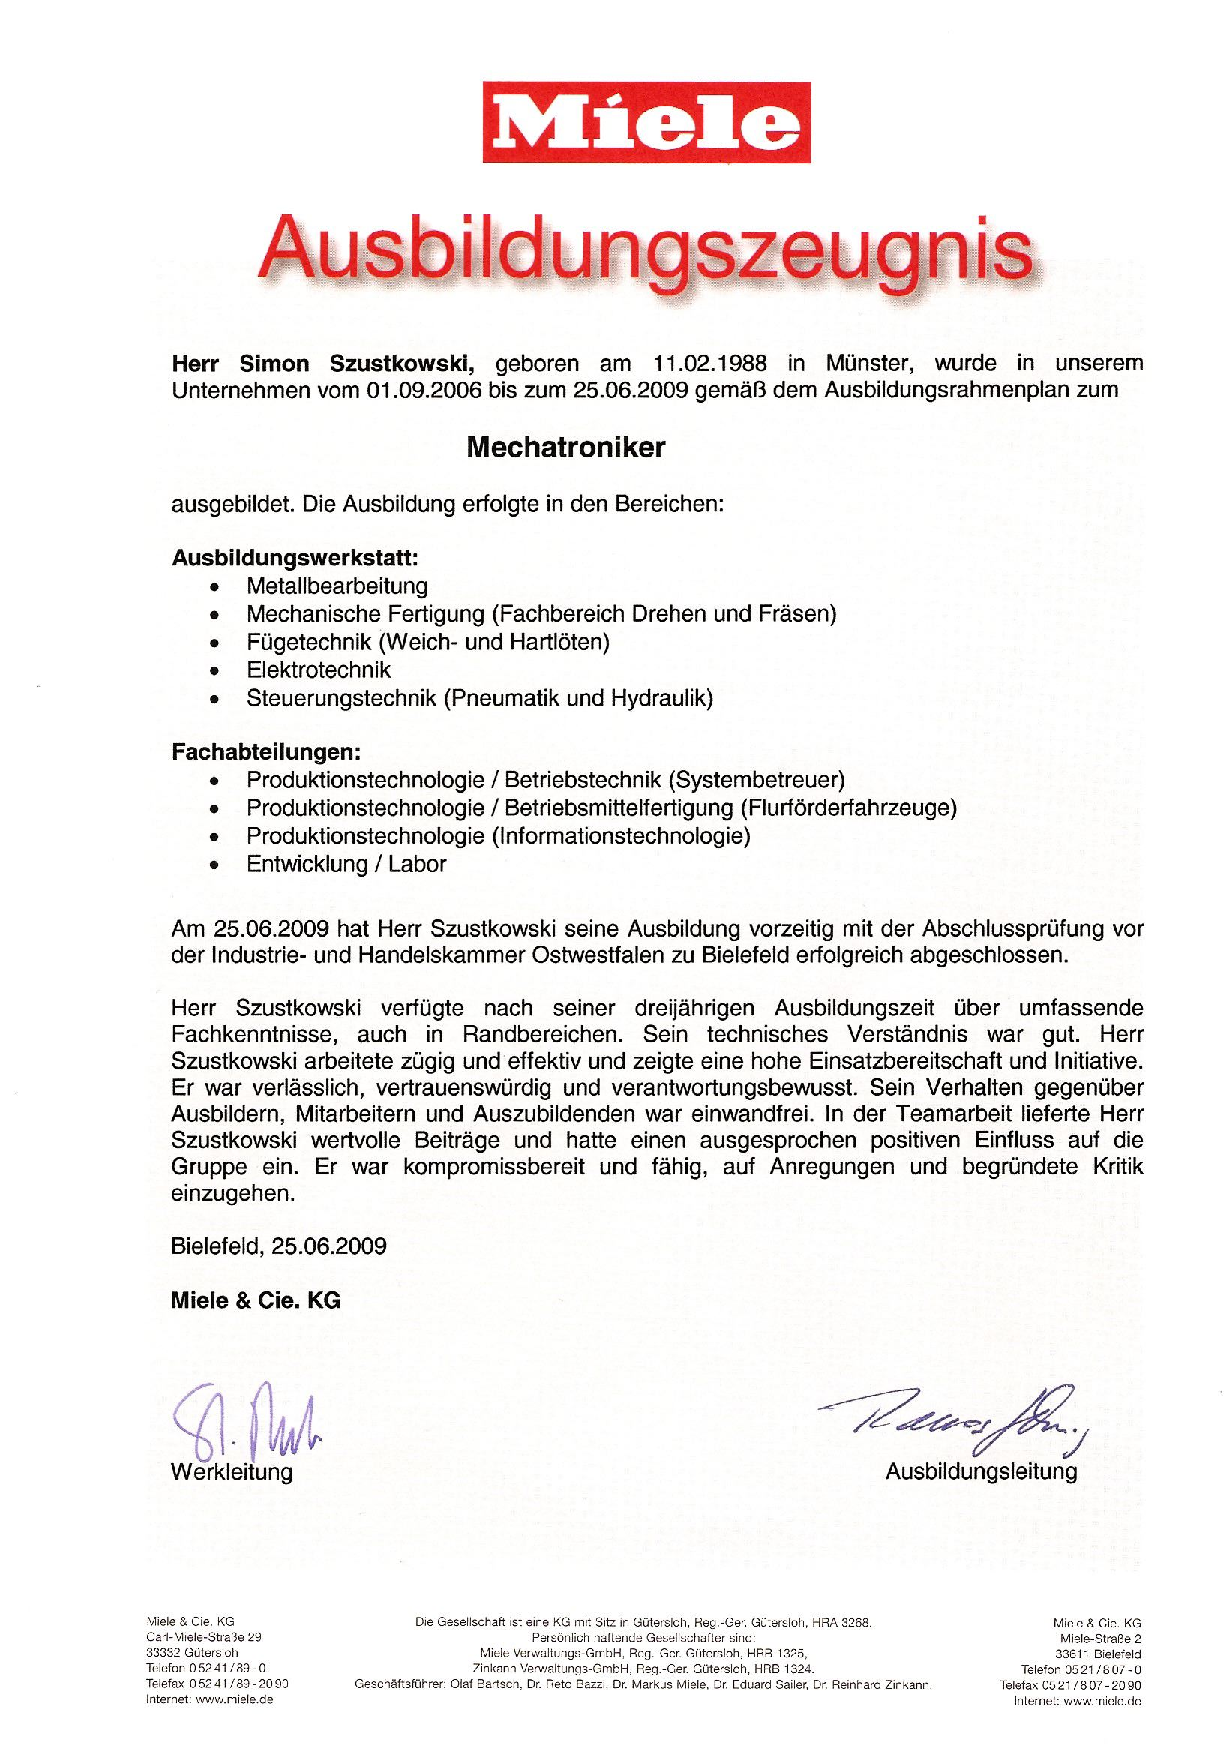
\includepdf[pages=1,addtotoc={1, section, 1, Arbeitszeugnis Miele \& Cie. KG, azmiele} ]{./Arbeitszeugnisse/Miele.pdf}


%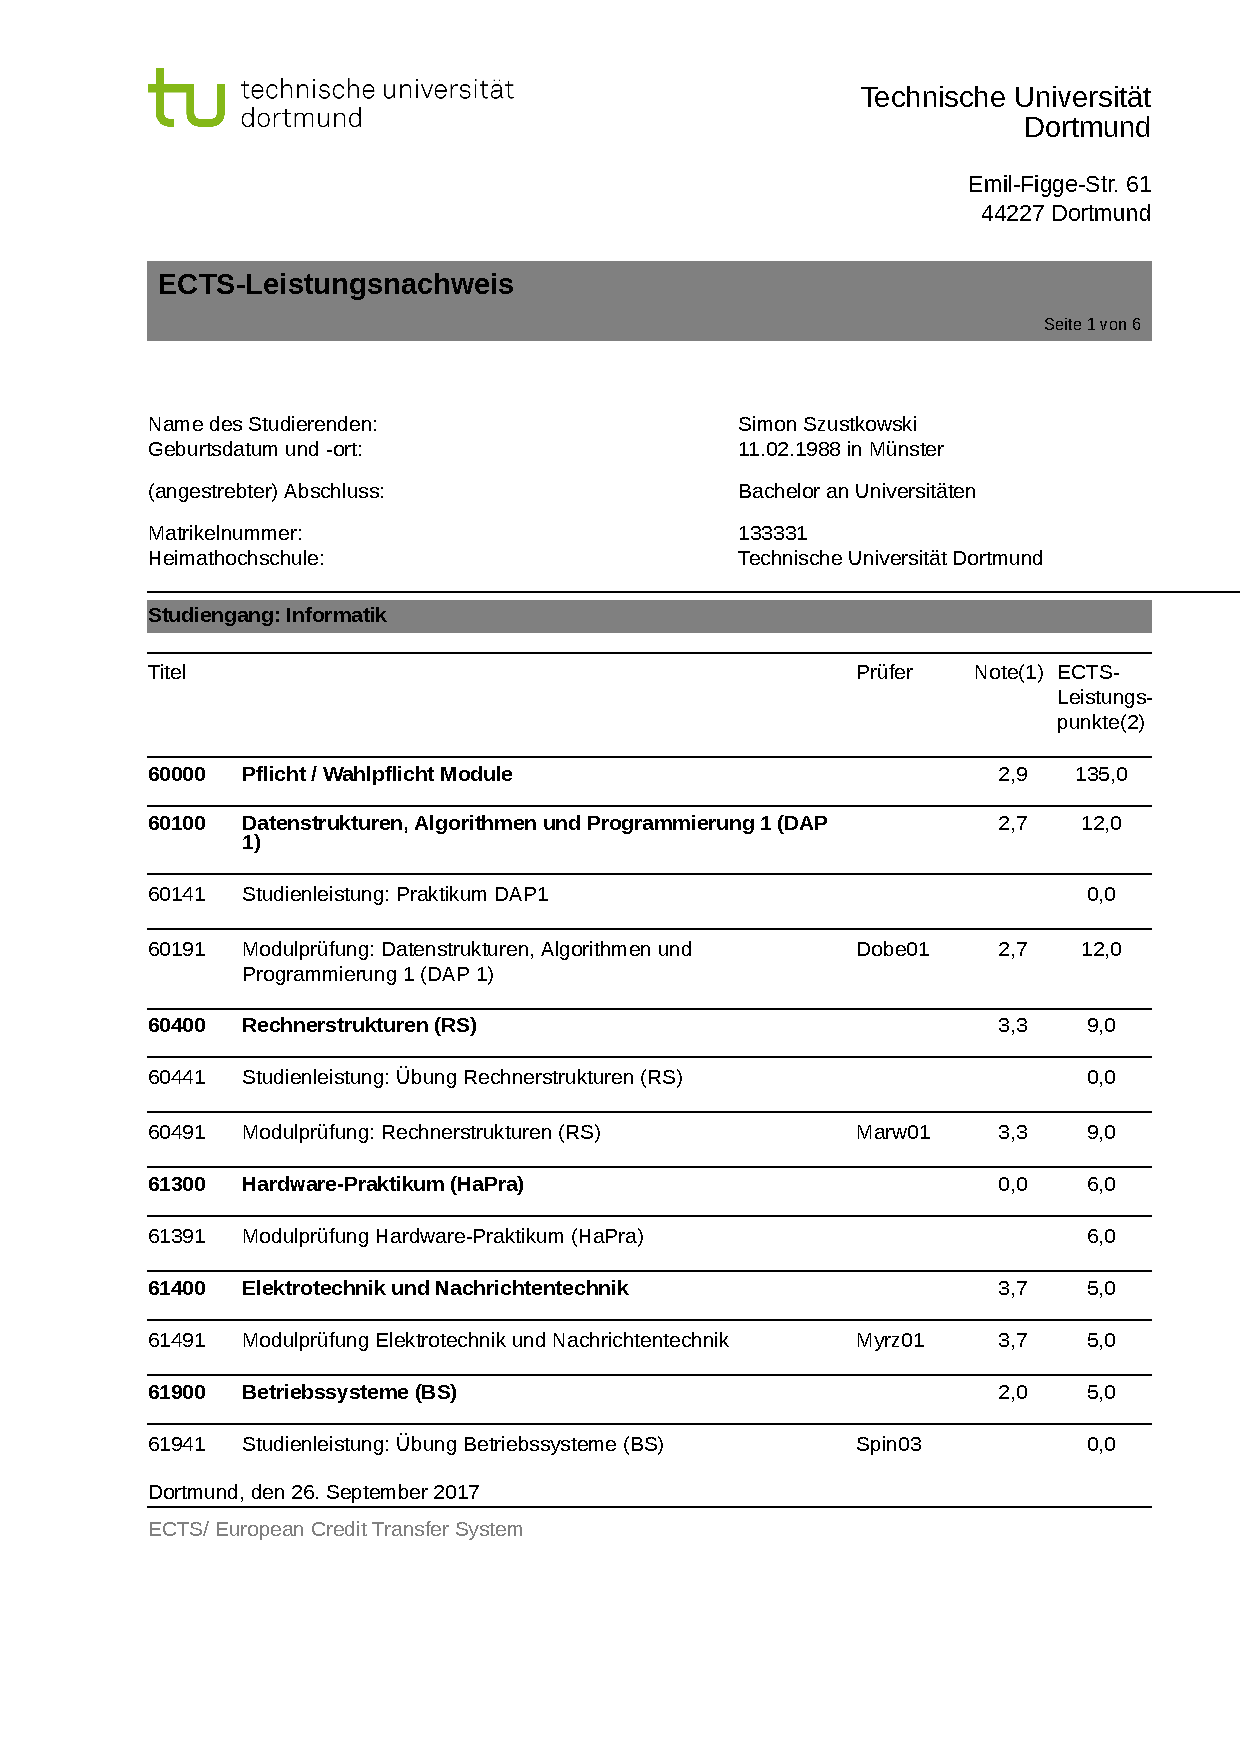
\includepdf[pages=1-,addtotoc={1, section, 1, Notenspiegel, notenspiegel} ]{notenspiegel.pdf}

%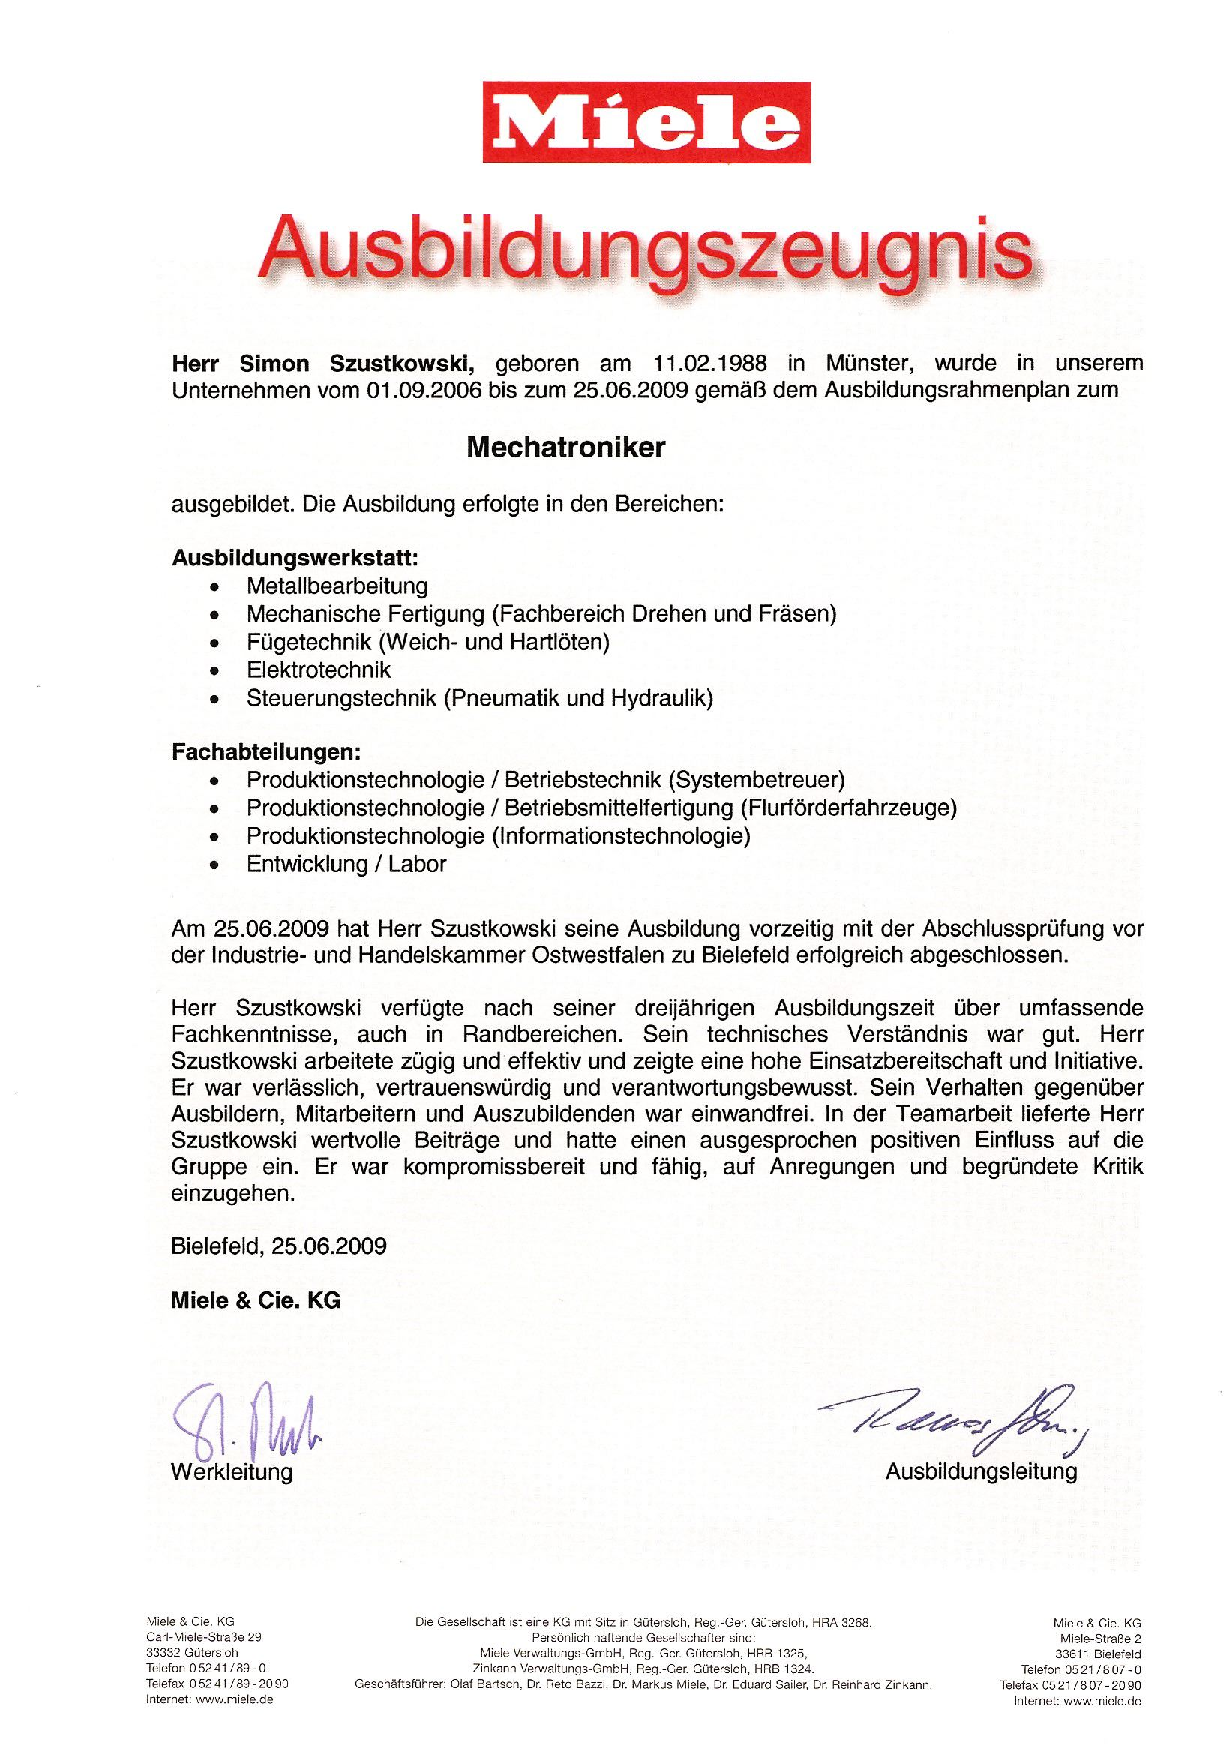
\includepdf[pages=1-,pagecommand={\chapter{Arbeitszeugnis Miele \& Cie. KG}}]{azmiele.pdf}
%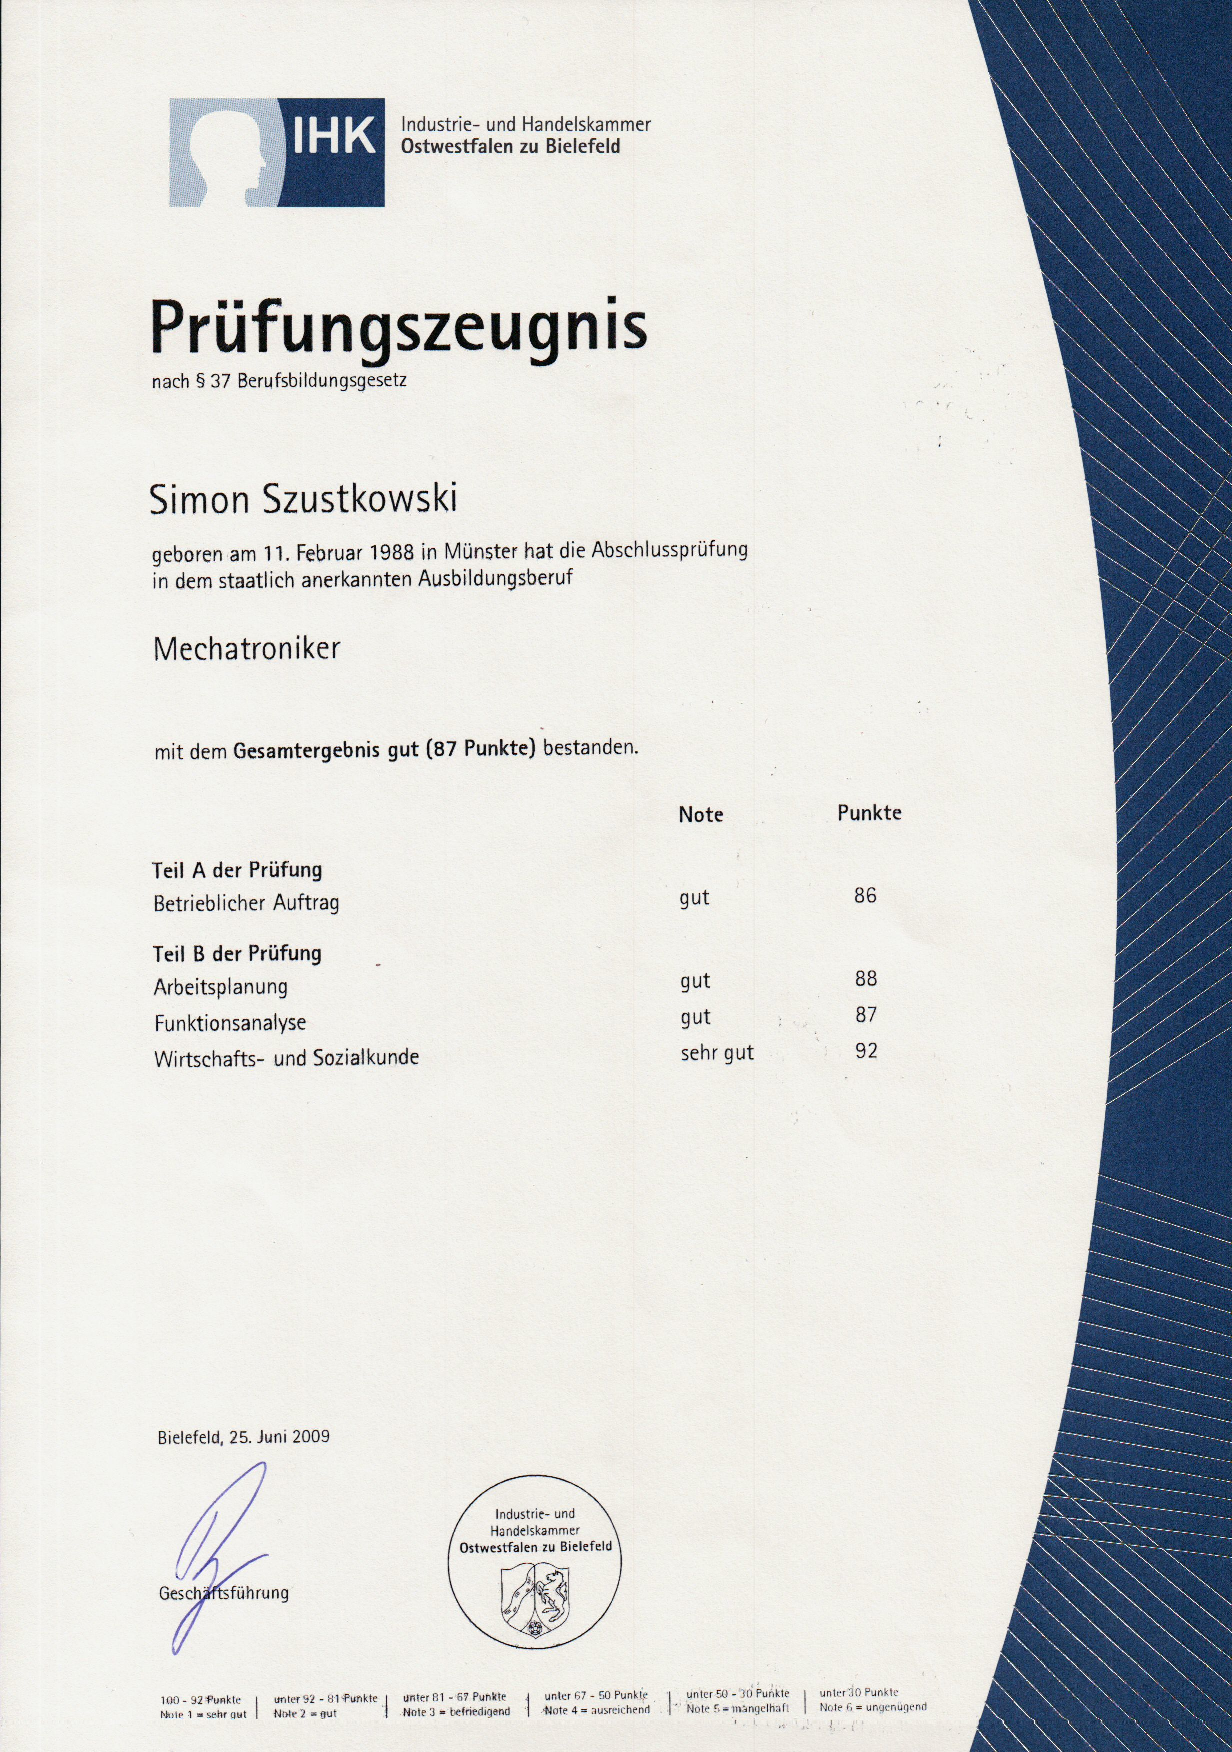
\includepdf[pages=1-]{ausbildungszeugnis.pdf}
%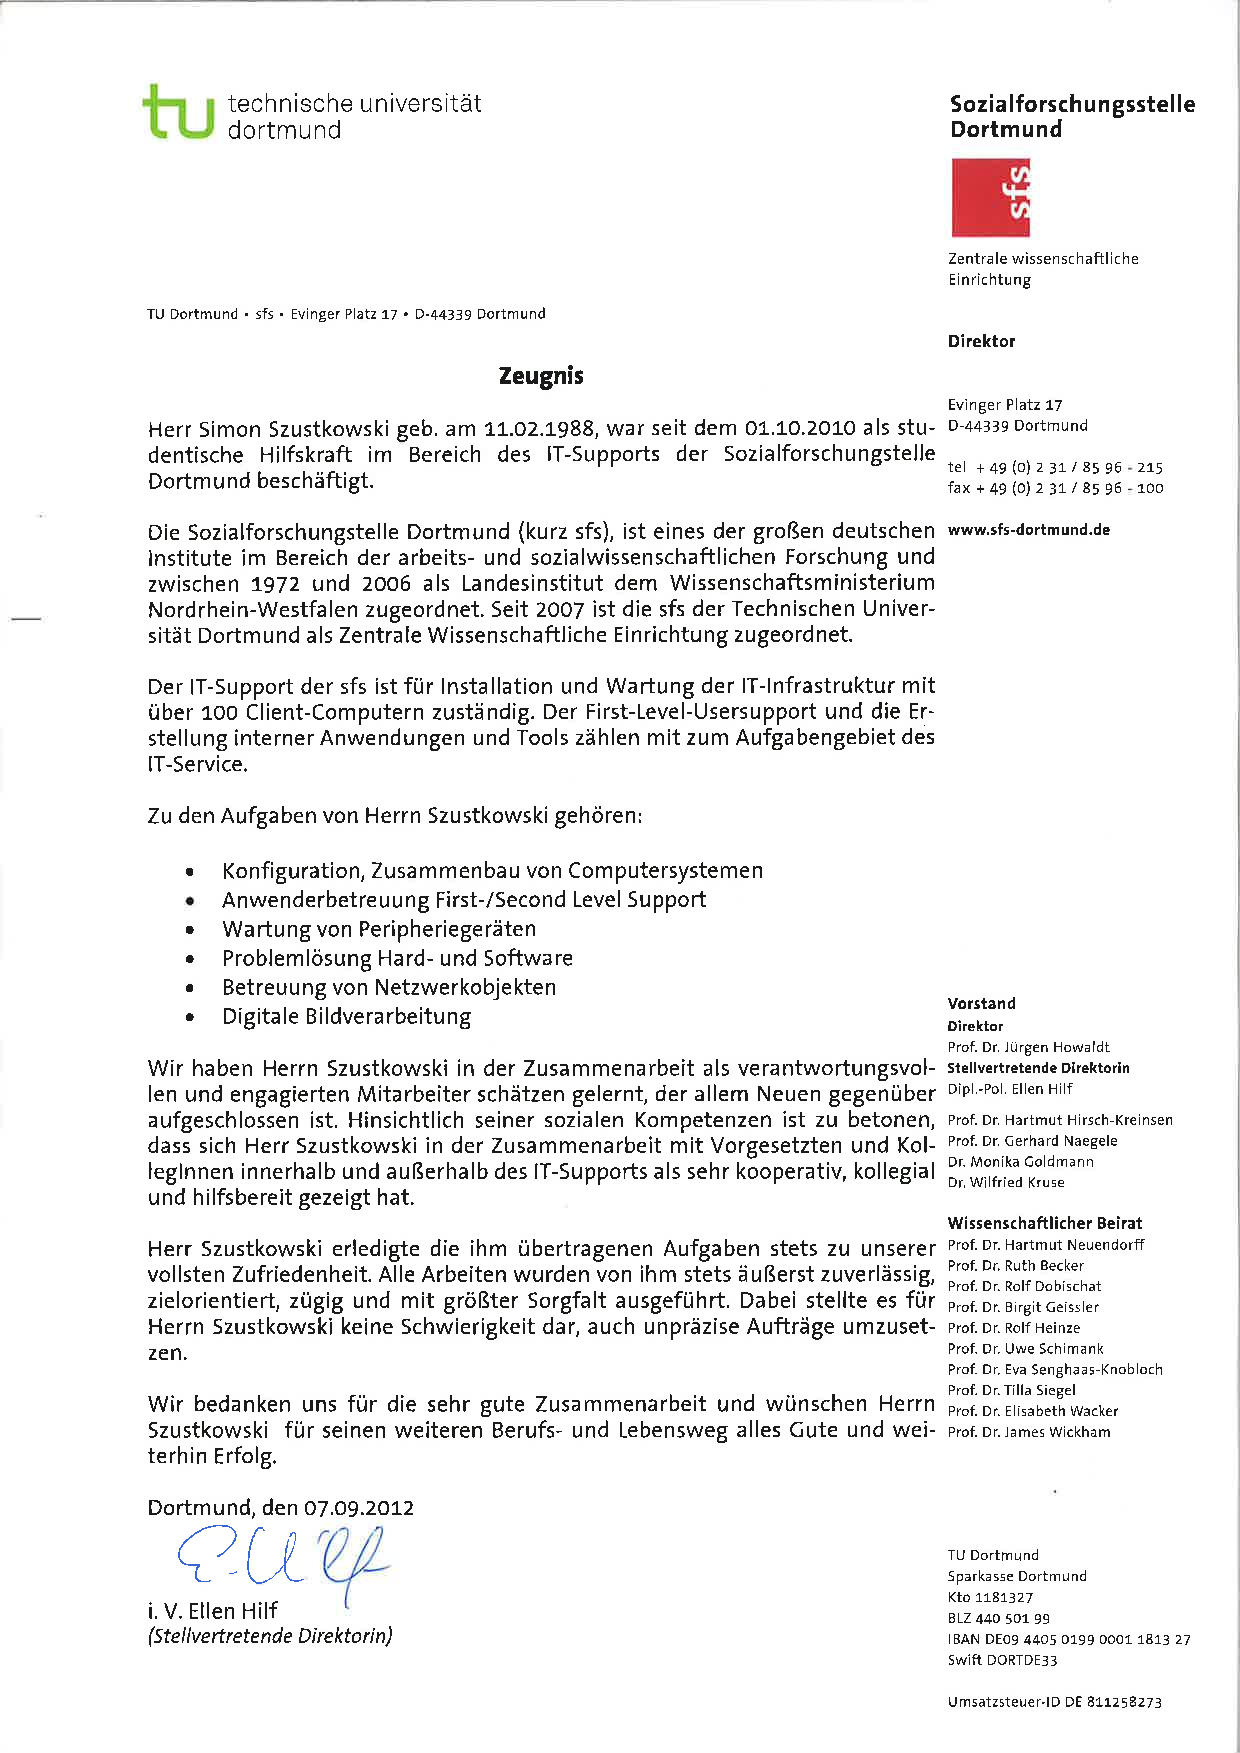
\includepdf[pages=1-]{azsfs.pdf}
%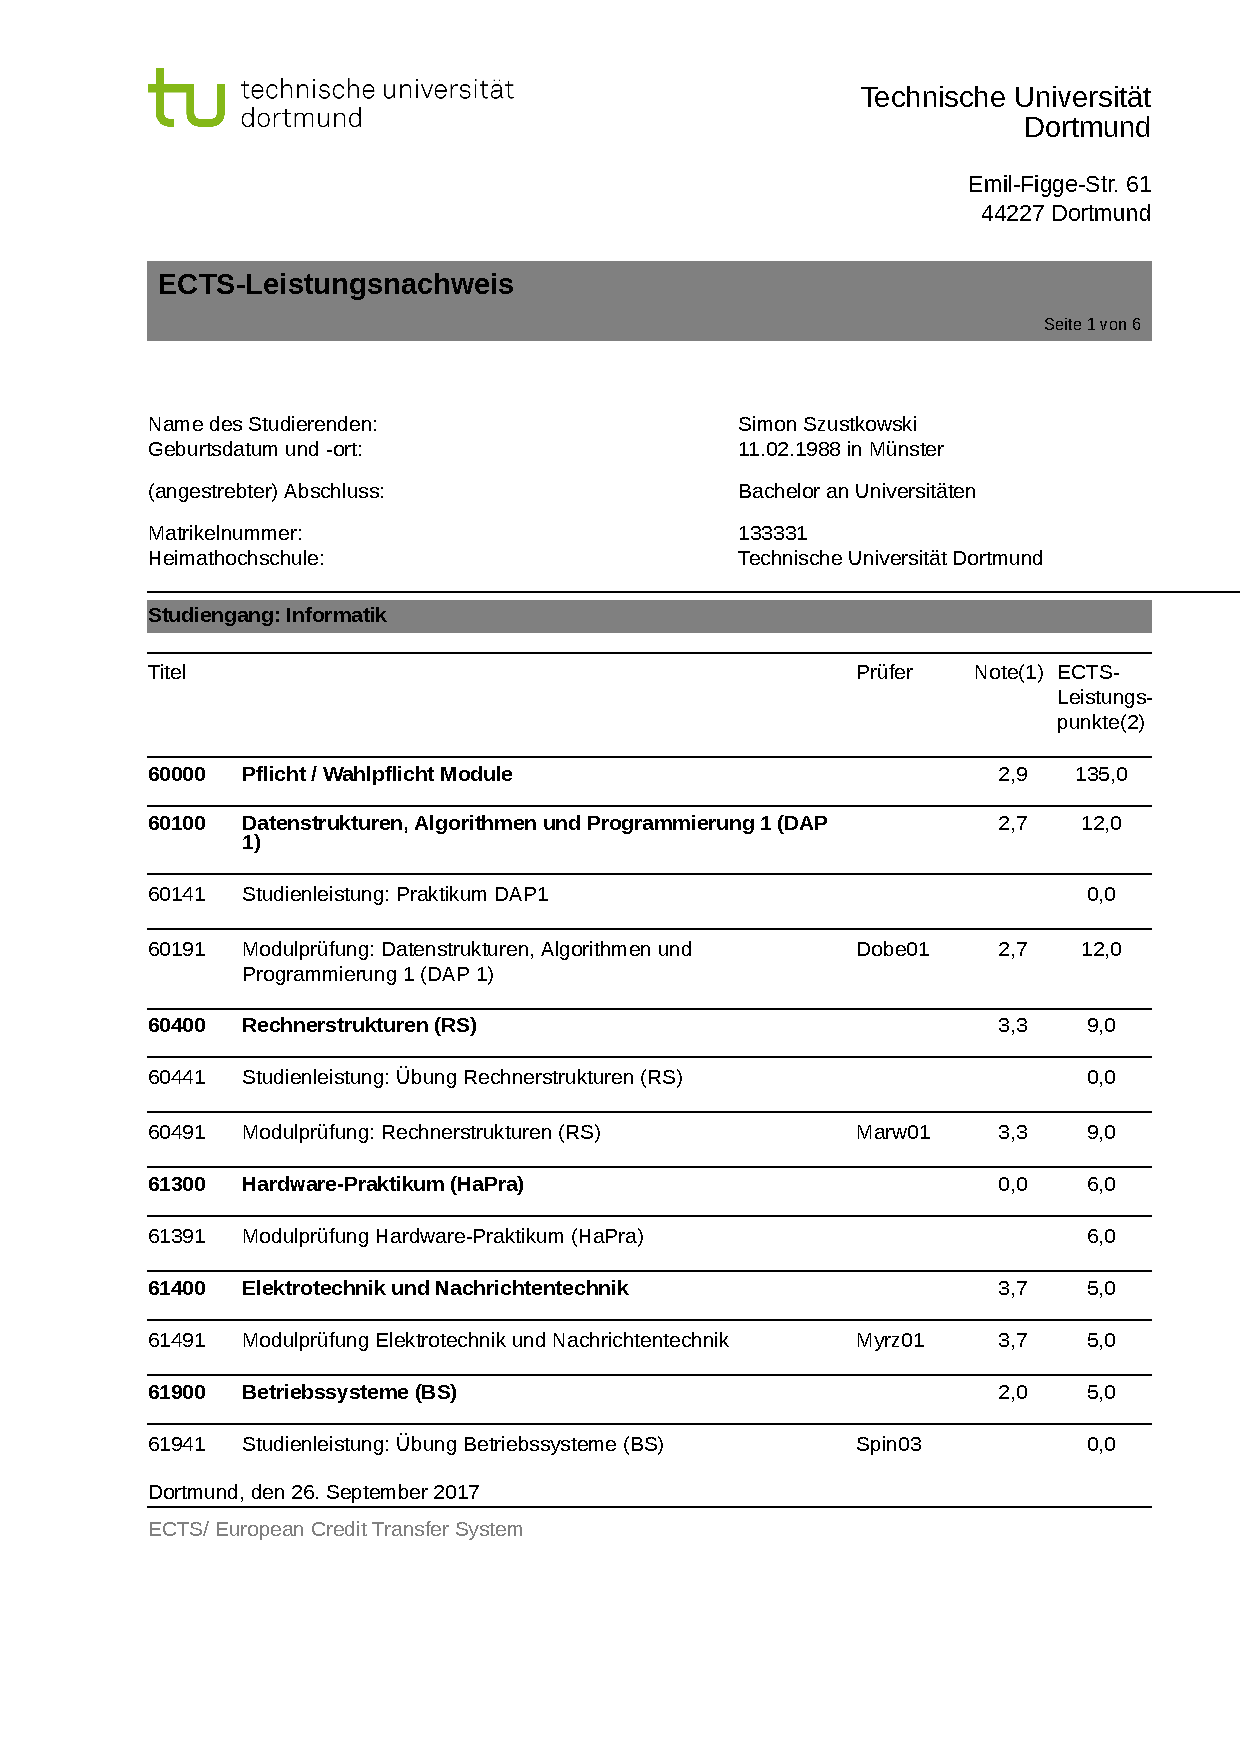
\includepdf[pages=1-]{notenspiegel.pdf}






%\chapter{Bachelor}{zeugnis}
%\vspace*{1cm}
%\begin{center}
	% \fbox{\includegraphics[height=0.85\textheight]{Bakk-Zeugnis}}	
%\end{center}

%\newpage
%\chapter{Master}{zeugnis}
%\vspace*{1cm}
%\begin{center}
	% \fbox{\includegraphics[height=0.85\textheight]{Masterzeugnis}}	
%\end{center}

%\vspace*{1cm}
%\begin{center}
	% \fbox{\includegraphics[height=0.85\textheight]{Masterzeugnis-2}}	
%\end{center}

% \newpage
% \chapter{Abschluss}{zeugnis}
% \vspace*{1cm}
% \begin{center}
% 	% \fbox{\includegraphics[height=0.85\textheight]{Abschlusszeugnis}}	
% \end{center}

\end{document}

% end of file `cv_german.tex'
